\documentclass[a4paper, 11pt]{book}
\usepackage{/home/nicolas/Documents/Enseignement/Prepa/bpep/fichiers_utiles/preambule}

\newcommand{\dsNB}{4}
\makeatletter
\renewcommand{\@chapapp}{Kh\^olles MPSI3 -- semaine \dsNB}
\makeatother

\toggletrue{corrige}  % décommenter pour passer en mode corrigé

\begin{document}

\resetQ
\newpage

\chapter{Sujet 1\siCorrige{\!\!-- corrig\'e}}
\section{Question de cours}

Démontrer les relations des ponts diviseurs de tension et de courant.

\subimport{/home/nicolas/Documents/Enseignement/Prepa/bpep/exercices/Colle/doublet_focal/}{sujet.tex}

\resetQ
\newpage

\chapter{Sujet 2\siCorrige{\!\!-- corrigé}}
\section{Question de cours}

\begin{minipage}{0.45\linewidth} Démontrer les relations des associations séries
    et parallèles et exprimer la résistance équivalente du circuit ci-contre.
\end{minipage}
\begin{minipage}{0.45\linewidth}
    \begin{center}
        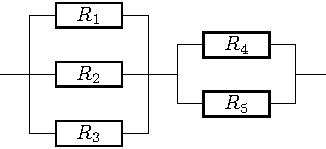
\includegraphics[width=\linewidth]{ch4-req}
    \end{center}
\end{minipage}

\subimport{/home/nicolas/Documents/Enseignement/Prepa/bpep/exercices/Colle/doublet_focal_2/}{sujet.tex}

\resetQ
\newpage

\chapter{Sujet 3\siCorrige{\!\!-- corrigé}}
\section{Question de cours}

Présenter et démontrer les caractéristiques d'un condensateur et d'une bobine~:
relation courant-tension (sans démonstration pour la bobine), continuité, régime
permanent, énergie stockée.

\subimport{/home/nicolas/Documents/Enseignement/Prepa/bpep/exercices/Colle/lunette_astronomique/}{sujet.tex}

\resetQ
\newpage

\chapter{Sujet 4\siCorrige{\!\!-- corrigé}}

\resetQ
\subimport{/home/nicolas/Documents/Enseignement/Prepa/bpep/exercices/Colle/teleobjectif/}{sujet.tex}
\subimport{/home/nicolas/Documents/Enseignement/Prepa/bpep/exercices/TD/deviation_3_miroirs/}{sujet.tex}

\end{document}
